\documentclass[theme=teal,16pt]{khmermath}
\usepackage{needspace}

\geometry{left=0.5cm, right=0.5cm, top=0.55cm, bottom=1.0cm, footskip=0.55cm}
\usepackage{colortbl}
\usepackage{tikz}
\usetikzlibrary{calc,shapes,arrows,intersections,through,backgrounds,shadows,decorations.pathmorphing,angles,quotes}

% Define arc accent
\newcommand{\wideparen}[1]{\overset{\boldsymbol{\frown}}{#1}}

% -------------------------------------------------------------------------
% Korean Math Textbook Style Color Palette & Macros
% -------------------------------------------------------------------------
\definecolor{koreaTeal}{RGB}{0, 150, 155}       % Primary Header Teal/Cyan
\definecolor{koreaDarkTeal}{RGB}{0, 105, 110}   % Dark Teal Accent
\definecolor{koreaBeige}{RGB}{247, 244, 237}     % Concept Sidebar Beige (#F7F4EE)
\definecolor{koreaBeigeBorder}{RGB}{225, 218, 205}
\definecolor{koreaOrange}{RGB}{235, 115, 30}     % Problem Number Orange
\definecolor{koreaBlue}{RGB}{35, 110, 190}      % Standard Blue
\definecolor{koreaPurple}{RGB}{125, 50, 160}    % Purple Accent
\definecolor{koreaNumber}{RGB}{115, 125, 135}   % Problem Number Gray
\definecolor{koreaYellow}{RGB}{255, 246, 175}   % Yellow Highlight Tint

\definecolor{brandNavy}{RGB}{0, 105, 110}
\definecolor{brandDarkTeal}{RGB}{0, 105, 110}
\definecolor{brandBlue}{RGB}{0, 150, 155}
\definecolor{brandLightBlue}{RGB}{247, 244, 237}
\definecolor{brandCrimson}{RGB}{195, 35, 60}
\definecolor{brandCoral}{RGB}{235, 80, 75}
\definecolor{brandGold}{RGB}{215, 130, 10}
\definecolor{brandGoldBg}{RGB}{255, 252, 242}
\definecolor{brandTeal}{RGB}{0, 150, 155}
\definecolor{brandTealBg}{RGB}{244, 252, 250}
\definecolor{subtleGray}{RGB}{246, 251, 249}
\definecolor{cardBorder}{RGB}{220, 212, 198}

% Custom Header & Footer setup (Korean Textbook Style)
\usepackage{fancyhdr}
\pagestyle{fancy}
\fancyhf{}
\renewcommand{\headrulewidth}{0pt}
\renewcommand{\footrule}{\color{koreaTeal!60}\hrule height 0.6pt\vspace{2pt}}

\fancyfoot[L]{%
  \fontsize{8.5}{8.5}\selectfont\kml \color{koreaNumber}\textbf{\thepage}\ \vline\ \color{koreaDarkTeal}\textbf{២. សមមាត្រ}%
}
\fancyfoot[C]{%
  \fontsize{8.5}{8.5}\selectfont\kby \color{koreaDarkTeal}\textbf{\ding{72}\ បង្រៀនដោយ ៖ \textcolor{koreaDarkTeal}{ក្រូត រស្មី}\ \ding{72}}%
}
\fancyfoot[R]{%
  \fontsize{8.5}{8.5}\selectfont\kby \color{koreaDarkTeal}\textbf{ Telegram: \textcolor{brandCrimson}{070897540}}\ \vline\ \color{koreaNumber}\textbf{\thepage}%
}

% Korean Header Banner
\newcommand{\koreanheader}[2]{%
  \noindent%
  \begin{tikzpicture}[x=1cm, y=1cm]
    \fill[koreaTeal, rounded corners=12pt] (0, 0.1) -- (0, 0.95) -- (3.8, 0.95) [rounded corners=0pt] -- (4.4, 0.1) -- cycle;
    \node[white, font=\fontsize{11}{11}\selectfont\kml\bfseries] at (1.9, 0.52) {#1};
    \node[anchor=west, font=\fontsize{15}{15}\selectfont\kml\bfseries, color=koreaDarkTeal] at (4.6, 0.42) {#2};
    \node[anchor=east, font=\fontsize{8.5}{8.5}\selectfont\kby, color=gray!80] at (19.4, 0.48) {$>$ ក្លឹបសិក្សាគណិតវិទ្យា ភី ស៊ី​ អឹម};
  \end{tikzpicture}%
  \vspace{2pt}%
}

% Yellow Formula Highlight Box
\newcommand{\koreahl}[1]{\colorbox{koreaYellow}{\fontsize{8.2}{8.2}\selectfont\textbf{#1}}}

% General Rule Box (Teal/Emerald Theme - ជាទូទៅ)
\newtcolorbox{khboxorange}[1][]{
  enhanced,
  colframe=brandNavy!40,
  colback=brandLightBlue,
  boxrule=0.7pt,
  arc=4.5pt,
  borderline west={3.5pt}{0pt}{brandNavy},
  drop fuzzy shadow=brandNavy!15,
  left=7pt, right=7pt, top=4pt, bottom=4pt,
  colupper=blue,
  title={\fontsize{8.5}{8.5}\selectfont\kml\color{white}\ding{72}\ ជាទូទៅ},
  coltitle=white,
  colbacktitle=brandNavy,
  boxed title style={
    boxrule=0pt,
    arc=3pt,
    left=5pt, right=5pt, top=1.5pt, bottom=1.5pt
  },
  attach boxed title to top left={yshift*=-\tcboxedtitleheight/2, xshift=10pt},
  before skip=4pt, after skip=4pt,
  #1
}

% Custom Title Rule Box
\newtcolorbox{khboxtitle}[2][]{
  enhanced,
  colframe=brandNavy!40,
  colback=brandLightBlue,
  boxrule=0.7pt,
  arc=4.5pt,
  borderline west={3.5pt}{0pt}{brandNavy},
  drop fuzzy shadow=brandNavy!15,
  left=7pt, right=7pt, top=4pt, bottom=4pt,
  colupper=blue,
  title={\fontsize{8.5}{8.5}\selectfont\kml\color{white}\ding{72}\ #2},
  coltitle=white,
  colbacktitle=brandNavy,
  boxed title style={
    boxrule=0pt,
    arc=3pt,
    left=5pt, right=5pt, top=1.5pt, bottom=1.5pt
  },
  attach boxed title to top left={yshift*=-\tcboxedtitleheight/2, xshift=10pt},
  before skip=4pt, after skip=4pt,
  #1
}

% Section Category Bar / Section Pill
\newcommand{\khtype}[1]{%
  \vspace{3.5pt}\noindent%
  \begin{tikzpicture}[baseline=(node.base)]
    \node[anchor=west, fill=brandCrimson, minimum width=3.5pt, minimum height=11pt, inner sep=0pt, rounded corners=1pt] at (0, 0) {};
    \node[anchor=west, font=\fontsize{9}{9}\selectfont\kml\bfseries, color=brandCrimson] (node) at (0.22, 0) {#1};
  \end{tikzpicture}\par\vspace{2pt}%
}

% Major Section Header with Dark Teal Badge
\newcommand{\khsection}[2]{%
  \vspace{2pt}\noindent%
  \begin{tikzpicture}[x=1cm, y=1cm]
    \node[fill=brandDarkTeal, text=white, font=\fontsize{9}{9}\selectfont\kml\bfseries, rounded corners=3pt, inner sep=2.5pt, minimum width=0.55cm, minimum height=0.5cm, align=center] (num) at (0.3, 0.25) {#1};
    \node[anchor=west, fill=brandDarkTeal!8, font=\fontsize{9.5}{9.5}\selectfont\kml\bfseries, text=brandCrimson, rounded corners=3pt, inner xsep=8pt, inner ysep=3.5pt, minimum height=0.55cm] at (0.68, 0.25) {#2};
  \end{tikzpicture}\par\vspace{2pt}%
}

% Korean Style Problem Number Pill: 01, 02...
\newcommand{\phead}[1]{%
  \tikz[baseline=(char.base)]\node[anchor=south west, text=koreaOrange, font=\fontsize{11}{11}\selectfont\kml\bfseries, inner sep=0pt] (char) {#1};%
  \hspace{3pt}%
}

% Korean Style Problem Number Pill with Self-Practice Badge
\newcommand{\pheadDIY}[1]{%
  \tikz[baseline=(char.base)]\node[anchor=south west, text=koreaOrange, font=\fontsize{11}{11}\selectfont\kml\bfseries, inner sep=0pt] (char) {#1};%
  \hspace{2pt}%
  \tikz[baseline=-0.3ex]\node[fill=brandCrimson!10, text=brandCrimson, draw=brandCrimson!35, line width=0.35pt, rounded corners=2pt, inner xsep=2.5pt, inner ysep=0.8pt, font=\fontsize{6}{6}\selectfont\kml\bfseries] {កិច្ចការធ្វើខ្លួនឯង};%
  \hspace{2.5pt}%
}

% Circular Khmer Letter Labels: ក, ខ, គ, ឃ...
\newcommand{\khlabel}[1]{%
  \tikz[baseline=(char.base)]\node[anchor=south west, fill=brandCrimson, text=white, rounded corners=2pt, inner xsep=2pt, inner ysep=0.8pt, font=\fontsize{7}{7}\selectfont\kml\bfseries] (char) {#1};%
  \hspace{1pt}%
}

% Small Note / Badge Pill
\newcommand{\khnote}[1]{%
  \tikz[baseline=(char.base)]\node[anchor=south west, fill=brandCrimson!10, text=brandCrimson, draw=brandCrimson!40, line width=0.4pt, rounded corners=2.5pt, inner xsep=3pt, inner ysep=1.2pt, font=\fontsize{7}{7}\selectfont\kml\bfseries] (char) {#1};%
}

% Small Concept Pill Badge
\newcommand{\khbadge}[1]{%
  \tikz[baseline=(char.base)]\node[anchor=south west, fill=brandTealBg, text=blue, draw=blue!30, line width=0.4pt, rounded corners=2.5pt, inner xsep=3.5pt, inner ysep=1.5pt, font=\fontsize{7.5}{7.5}\selectfont\kml\bfseries] (char) {#1};%
}

\makeatletter
\newcommand{\globalcolor}[1]{%
  \color{#1}\let\default@color\current@color
}
\makeatother
\AtBeginDocument{\globalcolor{blue}}

\setlength{\parindent}{0pt}
\setlength{\parskip}{2.5pt}
\setlength{\columnsep}{14pt}

\begin{document}
\globalcolor{black}
\fontsize{11}{11.8}\selectfont
\everymath{\color{blue}}
\everydisplay{\color{black}}

% =========================================================================
% TOPIC 1: សមមាត្រ (សមមាត្រស្រប និង ច្រាស) - PAGE 1
% =========================================================================
\koreanheader{មេរៀនទី ២}{សមមាត្រ}

\khsection{១}{ចំណោទដែលទាក់ទងនឹងសមមាត្រ (សមមាត្រស្រប និង ច្រាស)}
\color{blue}
យើងបានសិក្សារួចមកហើយប្រព័ន្ធរង្វាស់រង្វាល់ដែលយើងធ្លាប់ប្រើមាន $km$ សម្រាប់ចម្ងាយ និង $kg$ សម្រាប់ម៉ាសនៃវត្ថុ ។ ប៉ុន្តែនៅប្រទេសដទៃក៏មានរង្វាស់រង្វាល់ផ្សេងទៀត ដូចជា ម៉ាយ ($mile$) អ៊ីញ ($inch$) ហ្វីត ($feet$) សម្រាប់ចម្ងាយ និង ផោន ($lb$) សម្រាប់ម៉ាស ។

\begin{khboxtitle}[left=7pt, right=7pt, top=3pt, bottom=3pt, before skip=2pt, after skip=2pt]{មធ្យោបាយ និង វិធីសាស្រ្តបំបែកខ្នាត}
\color{blue}
% 1. Metric Conversion Chain (km ដល់ mm)
\noindent\textbf{\color{blue}\ding{226}\ ខ្នាតប្រវែងប្រព័ន្ធម៉ែត្រ (Metric Units ៖ $\text{km} \rightarrow \text{mm}$) ៖}\par\vspace{1pt}
\centerline{%
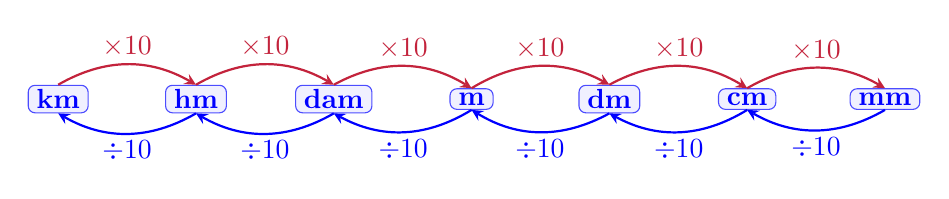
\begin{tikzpicture}[x=1.75cm, y=0.52cm]
  \foreach \u [count=\i] in {\mathbf{km}, \mathbf{hm}, \mathbf{dam}, \mathbf{m}, \mathbf{dm}, \mathbf{cm}, \mathbf{mm}} {
    \node[draw=blue!70, fill=blue!6, rounded corners=2.5pt, inner xsep=3pt, inner ysep=1.5pt, font=\fontsize{10}{7.5}\selectfont\color{blue}] (N\i) at (\i, 0) {$\u$};
  }
  \foreach \i [evaluate=\i as \next using int(\i+1)] in {1,...,6} {
    \draw[->, >=stealth, line width=0.8pt, brandCrimson] (N\i.north) to[bend left=30] node[midway, above=-1pt, font=\fontsize{10}{6}\selectfont\bfseries\color{brandCrimson}] {$\times 10$} (N\next.north);
    \draw[->, >=stealth, line width=0.8pt, blue] (N\next.south) to[bend left=30] node[midway, below=-1pt, font=\fontsize{10}{6}\selectfont\bfseries\color{blue}] {$\div 10$} (N\i.south);
  }
\end{tikzpicture}%
}
\vspace{1pt}\hrule height 0.3pt\vspace{2pt}

% 2. Imperial Conversion & General Rule
\begin{minipage}[c]{0.68\textwidth}
  \color{blue}
  \fontsize{10}{10.2}\selectfont
  \renewcommand{\arraystretch}{1.18}
  \begin{tabular}{@{}l@{\hspace{14pt}}l@{}}
    \textbf{\color{blue}\ding{226}\ រង្វាស់ប្រវែងអន្តរជាតិ (Imperial) ៖} & 
    \textbf{\color{blue}\ding{226}\ រង្វាស់ម៉ាស (Mass) ៖} \\
    $\star\ \mathbf{1\text{ ម៉ាយ (mile)}} \approx \mathbf{1.609\text{ km}}$ & $\star\ \mathbf{1\text{ ផោន (lb)}} \approx \mathbf{0.453\text{ kg}}$ \\
    $\star\ \mathbf{1\text{ អ៊ីញ (inch)}} = \mathbf{2.54\text{ cm}}$ & $\star\ \mathbf{1\text{ គីឡូក្រាម (kg)}} \approx \mathbf{2.205\text{ lb}}$ \\
    $\star\ \mathbf{1\text{ ហ្វីត (feet)}} = \mathbf{0.3048\text{ m}}$ & \textbf{\color{blue}\ding{226}\ វិធីសមមាត្រ ៖} $\dfrac{1\text{ A}}{x\text{ A}} = \dfrac{k\text{ B}}{y\text{ B}} \implies y = x \times k$
  \end{tabular}
\end{minipage}\hfill
\begin{minipage}[c]{0.30\textwidth}
  \centering
  \begin{tikzpicture}[scale=1, every node/.style={scale=0.72}]
    \node[draw=blue, fill=blue!8, rounded corners=3.5pt, inner sep=3pt, font=\fontsize{10}{7.5}\selectfont\kml\bfseries\color{blue}] (A) at (0,0) {ខ្នាតធំ};
    \node[draw=blue, fill=blue!8, rounded corners=3.5pt, inner sep=3pt, font=\fontsize{10}{7.5}\selectfont\kml\bfseries\color{blue}] (B) at (2.5,0) {ខ្នាតតូច};
    \draw[->, >=stealth, line width=1pt, brandCrimson] (A.north) to[bend left=35] node[midway, above, font=\fontsize{10}{6.5}\selectfont\bfseries\color{brandCrimson}] {$\times k$ (គុណ)} (B.north);
    \draw[->, >=stealth, line width=1pt, blue] (B.south) to[bend left=35] node[midway, below, font=\fontsize{10}{6.5}\selectfont\bfseries\color{blue}] {$\div k$ (ចែក)} (A.south);
  \end{tikzpicture}\par\vspace{1pt}
  \fontsize{10}{7}\selectfont\kml\color{blue}{\textbf{\ding{72}\ $\text{in} \xrightarrow{\times 2.54} \text{cm} \;\mid\; \text{cm} \xrightarrow{\div 2.54} \text{in}$}}
\end{minipage}
\end{khboxtitle}

\begin{khboxorange}
\begin{minipage}[c]{0.68\textwidth}
  \fontsize{12}{10.5}\selectfont
  \begin{itemize}[leftmargin=10pt, itemsep=1pt]
    \item \textbf{សមមាត្រស្រប ៖} $\dfrac{y}{x} = k \iff \dfrac{x_1}{y_1} = \dfrac{x_2}{y_2}$ ($x\text{ កើន } \Longrightarrow y\text{ កើន}$)
    \item \textbf{សមមាត្រច្រាស ៖} $x \cdot y = k \iff \koreahl{$x_1 y_1 = x_2 y_2$}$ ($x\text{ កើន } \Longrightarrow y\text{ ថយ}$)
    \item \textbf{លក្ខណៈគ្រឹះ ៖} $\dfrac{a}{b} = \dfrac{c}{d} \iff ad = bc \implies a = \dfrac{bc}{d},\; d = \dfrac{bc}{a}$
  \end{itemize}
\end{minipage}\hfill
\begin{minipage}[c]{0.30\textwidth}
  \centering
  \begin{tikzpicture}[scale=1.2, every node/.style={scale=1}]
    \node[draw=brandDarkTeal, fill=white, rounded corners=3pt, inner sep=2.5pt, font=\fontsize{7.5}{7.5}\selectfont\bfseries\color{brandDarkTeal}] at (0, 0.45) {សមមាត្រស្រប ៖ $\frac{x_1}{y_1} = \frac{x_2}{y_2}$};
    \node[draw=brandCrimson, fill=brandCrimson!6, rounded corners=3pt, inner sep=2.5pt, font=\fontsize{7.5}{7.5}\selectfont\bfseries\color{brandCrimson}] at (0, -0.2) {សមមាត្រច្រាស ៖ $x_1 y_1 = x_2 y_2$};
  \end{tikzpicture}
\end{minipage}
\end{khboxorange}

\begin{multicols}{2}

\khtype{ប្រភេទទី ១ ៖ ការប្ដូរខ្នាតប្រាស់ប្រាស់}
\noindent\phead{01} \textbf{ចូរ​ប្តូរ​ខ្នាត​នីមួយៗ​ខាងក្រោម ៖}
\vspace{-0.5cm}
\begin{multicols}{2}
\khlabel{ក} $5\text{in} \rightarrow \text{cm}$ \\
\khlabel{ខ} $12.5\text{in} \rightarrow \text{cm}$ \\
\khlabel{គ} $5\text{cm} \rightarrow \text{in}$ \\
\khlabel{ឃ} $20\text{cm} \rightarrow \text{in}$ \\
\khlabel{ង} $1\text{m} \rightarrow \text{in}$ \\
\khlabel{ច} $100\text{km} \rightarrow \text{mile}$ \\
\khlabel{ឆ} $5\text{mile} \rightarrow \text{km}$ \\
\khlabel{ជ} $6\text{ft} \rightarrow \text{m}$ \\
\khlabel{ឈ} $1\text{kg} \rightarrow \text{lb}$ \\
\khlabel{ញ} $100\text{lb} \rightarrow \text{kg}$
\end{multicols}
\vspace{-0.3cm}
\noindent\phead{02} \textbf{ពិសិដ្ឋ​មាន​កម្ពស់ $175\text{cm}$ តើ​កម្ពស់​របស់​គាត់​ត្រូវជា​ប៉ុន្មាន​អ៊ីញ?}

\noindent\pheadDIY{03}\textbf{ចូរ​ប្តូរ $8\text{inch}$ ទៅជា $\text{cm}$ និង $50\text{cm}$ ទៅជា $\text{inch}$ ។}

\noindent\pheadDIY{04} \textbf{ចម្ងាយ​ផ្លូវ​ពី​ផ្ទះ​ទៅ​សាលាគឺ $3.218\text{km}$ ។ តើ​ត្រូវជា​ប៉ុន្មាន​ម៉ាយ ($\text{mile}$)?}

\noindent\pheadDIY{05}\textbf{ថង់​អង្ករ​មួយ​មាន​ម៉ាស $45\text{kg}$ ។ តើ​មាន​ម៉ាស​ប៉ុន្មាន​ផោន ($\text{lb}$)?}

\khtype{ប្រភេទទី ២ ៖ សមមាត្រស្រប}

\noindent\phead{06} \textbf{ទិញ​ផ្លែដូង $14$ ផ្លែអស់ប្រាក់ $32\,200$ រៀល ប្រសិន​បើ​មាន​ប្រាក់ $41\,400$ រៀល តើ​អាច​ទិញ​ដូង​បាន​ប៉ុន្មាន​ផ្លែ? បើ​តម្លៃ​ដូង​ស្មើគ្នា ។}

\noindent\phead{07} \textbf{អាង​ទឹក​មួយ​ចំណុះ $7650\text{dm}^3$ បើ​បញ្ចូល​ទឹក​ក្នុង​ល្បឿន $85\text{dm}^3$ ក្នុង $2$ នាទី តើ​ត្រូវ​ប្រើ​ពេល​ប៉ុន្មាន​ទើប​ពេញ​អាង?}


\noindent\phead{08} \textbf{បើ​កង់​មួយ​វិល​បាន $1750$ ជុំក្នុងរយៈពេល $5$ វិនាទី តើ​ក្នុង​រយៈពេល​មួយ​ម៉ោង ($3600$ វិនាទី) វា​វិល​បាន​ប៉ុន្មាន​ជុំ?}




\noindent\pheadDIY{09} \textbf{សៀវភៅសរសេរ $8$ ក្បាលថ្លៃ $24\,000$ រៀល ។ បើទិញ $15$ ក្បាល តើត្រូវអស់ប្រាក់ប៉ុន្មាន?}

\noindent\pheadDIY{10} \textbf{ទុយោមួយបង្ហូរទឹកបាន $120\text{L}$ ក្នុង $3$ នាទី ។ តើត្រូវប្រើពេលប៉ុន្មានដើម្បីបង្ហូរបាន $800\text{L}$ ពេញអាង?}

\noindent\pheadDIY{11} \textbf{ម៉ាស៊ីនបោះពុម្ពមួយបោះបាន $450$ ទំព័រក្នុង $6$ នាទី ។ តើក្នុង $15$ នាទី បោះបានប៉ុន្មានទំព័រ?}\\
\khtype{ប្រភេទទី ៣ ៖ សមមាត្រច្រាស}
\noindent\phead{12} \textbf{កម្មករ $6$ នាក់​សង់​រោង​មួយ​រួច​ក្នុង​ពេល $8$ ថ្ងៃ ។ ប្រសិន​បើ​បន្ថែម​កម្មករ $2$ នាក់​ទៀត (សរុប $8$ នាក់) តើ​ត្រូវ​ប្រើ​ពេល​ប៉ុន្មាន​ថ្ងៃ​ទើប​សង់​រួច?}

\noindent\phead{13} \textbf{រថយន្ត​មួយ​បើក​ល្បឿន​មធ្យម $60\text{km/h}$ ពី​ភ្នំពេញ​ទៅ​កំពង់សោម​ប្រើ​ពេល $4$ ម៉ោង ។ ប្រសិន​បើ​បង្កើន​ល្បឿន​ដល់ $80\text{km/h}$ តើ​ប្រើ​ពេល​ប៉ុន្មាន​ម៉ោង?}

\noindent\phead{14} \textbf{ម៉ាស៊ីន​បូម​ទឹក $3$ គ្រឿង​បូម​ទឹក​អស់​ក្នុង​ពេល $40$ នាទី ។ បើ​ប្រើ​ម៉ាស៊ីន $4$ គ្រឿង​កម្លាំង​ស្មើគ្នា តើ​ត្រូវ​ប្រើ​ពេល​ប៉ុន្មាន​នាទី​ទើប​បូម​អស់?}


\noindent\pheadDIY{15} \textbf{កម្មករ $4$ នាក់ច្រូតស្រូវលើដីស្រែមួយរួចក្នុងពេល $6$ ថ្ងៃ ។ បើប្រើកម្មករ $8$ នាក់វិញ តើត្រូវប្រើពេលប៉ុន្មានថ្ងៃ?}

\noindent\pheadDIY{16} \textbf{ម៉ូតូមួយបើកដោយល្បឿន $40\text{km/h}$ ប្រើពេល $3$ ម៉ោងដល់គោលដៅ ។ បើចង់ដល់ក្នុងពេល $2$ ម៉ោង តើត្រូវបើកល្បឿនប៉ុន្មាន?}

\noindent\pheadDIY{17} \textbf{ម៉ាស៊ីនត្រជាក់ $2$ គ្រឿងប្រើពេល $30$ នាទីដើម្បីបញ្ចុះកម្តៅបន្ទប់ប្រជុំ ។ បើប្រើ $3$ គ្រឿង តើប្រើពេលប៉ុន្មាននាទី?}
\par\vspace{1pt}\centerline{\khbadge{$2\text{ គ្រឿង} \times 30\text{ នាទី} = 3\text{ គ្រឿង} \times t \implies t = 20\text{ នាទី}$}}\par\vspace{1pt}

\end{multicols}


% =========================================================================
% TOPIC 2: ភាគរយ (PERCENTAGE) - PAGE 2
% =========================================================================
\khsection{២}{ចំណោទដែលទាក់ទងនឹងភាគរយ}

\begin{khboxorange}
\begin{minipage}[c]{0.75\textwidth}
  \fontsize{11}{10.5}\selectfont
  \begin{itemize}[leftmargin=10pt, itemsep=1.5pt]
    \item \textbf{ភាគរយ (Percentage) ៖} គឺជាប្រភាគដែលមានភាគបែងស្មើ $100$ (សរសេរ $\frac{30}{100} = 30\%$)។
    \item \textbf{រូបមន្តគណនាភាគរយ ៖} ធៀបផ្នែក $a$ ទៅនឹងទំហំសរុប $b$ ៖
    $\koreahl{$P\% = \dfrac{a}{b} \times 100\%$}$
    \item \textbf{ការទាញរកតម្លៃ ៖}
    \begin{itemize}[leftmargin=8pt, itemsep=0.5pt]
      \item \textbf{រកផ្នែក $a$ ៖} $a = \dfrac{P}{100} \times b$
      \item \textbf{រកទំហំសរុប $b$ ៖} $b = \dfrac{a \times 100}{P}$
    \end{itemize}
  \end{itemize}
\end{minipage}\hfill

\end{khboxorange}

\begin{multicols}{2}

\khtype{ប្រភេទទី ១ ៖ ការគណនាតម្លៃភាគរយគ្រឹះ (ស្វែងរក $n$)}

\noindent\phead{01} \textbf{គណនា $n$ ដែល ៖}
\begin{multicols}{2}
\khlabel{ក} $30\%\text{ នៃ }n\text{ ស្មើ }48$ \\
\khlabel{ខ} $15\%\text{ នៃ }n\text{ ស្មើ }75$ \\
\khlabel{គ} $25\%\text{ នៃ }28\text{ ស្មើ }n$ \\
\khlabel{ឃ} $17\text{ ជា }n\%\text{ នៃ }85$ \\
\khlabel{ង} $n\%\text{ នៃ }150\text{ ស្មើ }20$ \\
\khlabel{ច} $n\text{ ស្មើ }30\%\text{ នៃ }400$
\end{multicols}

\noindent\pheadDIY{02} \textbf{គណនា $n$ ដែល ៖} \\
\khlabel{ក} $20\%\text{ នៃ }n\text{ ស្មើ }60$ \hfill \khlabel{ខ} $35\%\text{ នៃ }80\text{ ស្មើ }n$

\noindent\pheadDIY{03} \textbf{គណនា $n$ ដែល ៖} \\
\khlabel{ក} $n\%\text{ នៃ }200\text{ ស្មើ }50$ \hfill \khlabel{ខ} $18\text{ ជា }n\%\text{ នៃ }90$

\noindent\pheadDIY{04} \textbf{គណនា $n$ ដែល ៖} \\
\khlabel{ក} $n\text{ ស្មើ }45\%\text{ នៃ }800$ \hfill \khlabel{ខ} $75\%\text{ នៃ }n\text{ ស្មើ }150$

\khtype{ប្រភេទទី ២ ៖ ការគណនាភាគរយនៃបរិមាណ}

\noindent\phead{05} \textbf{តេស្ត​មួយ​មាន $20$ សំណួរ នីតា​ធ្វើ​ត្រូវ​បាន $17$ សំណួរ ។ រក​ភាគរយ​នៃ​សំណួរ​ដែល​ធ្វើត្រូវ ។}


\noindent\phead{06} \textbf{វីរៈ​រក​ប្រាក់​បាន $300\,000\text{ ៛}$ ក្នុង​មួយ​ខែ ហើយ​សន្សំ​ទុក​បាន $60\,000\text{ ៛}$ រក​ភាគរយ​នៃ​ប្រាក់​ដែល​វីរៈ​បាន​សន្សំ​ទុក ។}


\noindent\pheadDIY{07} \textbf{ក្នុងថ្នាក់រៀនមួយមានសិស្ស $40$ នាក់ ស្រី $24$ នាក់ ។ រកភាគរយនៃសិស្សស្រី ។}

\noindent\pheadDIY{08} \textbf{កសិករម្នាក់ប្រមូលស្រូវបាន $500\text{kg}$ ទុកហូប $125\text{kg}$ ។ រកភាគរយស្រូវទុកហូប ។}

\noindent\pheadDIY{09} \textbf{ការប្រឡងមួយមាន $50$ សំណួរ សុខាឆ្លើយត្រូវ $42$ សំណួរ ។ រកភាគរយឆ្លើយត្រូវ ។}




\khtype{ប្រភេទទី ៣ ៖ ចំណោទភាគរយនៃតម្លៃ និងកម្រៃជើងសារ}

\noindent\phead{10} \textbf{វណ្ណា​ចង់​ទិញ​កង់​មួយ​មាន​តម្លៃ $350\,000\text{ រៀល}$ ឥឡូវ​នេះ​គាត់​សន្សំ​បាន $60\%$ នៃ​តម្លៃ​កង់​រួចហើយ ។ តើ​គាត់​ខ្វះ​ប្រាក់​ប៉ុន្មាន​ទៀត​ទើប​ទិញ​កង់​នោះ​បាន ?}


\noindent\phead{11} \textbf{សុខ​ត្រូវ​រក​ប្រាក់​ឱ្យ​បាន $35\text{ លានរៀល}$ សម្រាប់​សង់​លំនៅដ្ឋាន​មួយ ឥឡូវ​នេះ​គាត់​សន្សំ​បាន $60\%\text{ នៃប្រាក់នេះ}$ ហើយ ។ រក​ប្រាក់​ដែល​គាត់​សន្សំ​បាន ? តើ​គាត់​ខ្វះ​ប្រាក់​ប៉ុន្មាន​ទៀត ?}
\begin{center}
\begin{tikzpicture}[scale=0.55, every node/.style={scale=0.62}]
  \draw[fill=brandTealBg, draw=brandNavy, thick] (0,0) rectangle (1.4,0.9);
  \draw[fill=brandCoral!30, draw=brandCoral, thick] (-0.2,0.9) -- (0.7,1.5) -- (1.6,0.9) -- cycle;
  \draw[fill=brandNavy, draw=brandNavy] (0.45,0) rectangle (0.95,0.5);
  \node[below, font=\fontsize{6}{6}\selectfont\kml\bfseries\color{brandNavy}] at (0.7,-0.05) {សន្សំបាន $60\%$ ($35$ លាន)};
\end{tikzpicture}
\end{center}

\noindent\phead{12} \textbf{សុខ​សន្សំ​បាន​ប្រាក់ $60\$$ ដែល​ត្រូវជា $80\%\text{ នៃតម្លៃម៉ាស៊ីនថត}$ រូប ។ រក​តម្លៃ​ម៉ាស៊ីន​នោះ​ថ្លៃ​ប៉ុន្មាន ?}
\par\vspace{1pt}\centerline{\khbadge{សន្សំ $60\$ = 80\% \implies \text{តម្លៃពេញ } 100\% = 75\$$}}\par\vspace{1pt}

\noindent\phead{13} \textbf{ក្រុមហ៊ុន​អចលនទ្រព្យ​លក់​ដី​ឱ្យ​គេ​ដោយ​ទទួល​បាន​ប្រាក់កម្រៃ $1\,800\$$ ត្រូវជា $3\%\text{ នៃថ្លៃដី}$ ។ តើ​ដី​ដែល​ត្រូវ​លក់​ថ្លៃ​ប៉ុន្មាន ?}
\par\vspace{1pt}\centerline{\khbadge{កម្រៃ $1\,800\$ = 3\% \implies \text{ថ្លៃដីសរុប } 100\% = 60\,000\$$}}\par\vspace{1pt}

\noindent\phead{14} \textbf{ក្រុមហ៊ុន​ឱ្យ​ប្រាក់កម្រៃ​ទៅ​ឧត្តម​ចំនួន $10\%\text{ នៃប្រាក់ដែលបានលក់}$ ហើយ​ឧត្តម​ចែក​ទៅ​ឡៃយី​ចំនួន $20\%\text{ នៃប្រាក់ទទួលបាន}$ ។ តើ​ឡៃយី​ទទួល​បាន​ប៉ុន្មាន បើ​ប្រាក់​លក់​បាន $4\text{ លានរៀល}$ ?}
\par\vspace{1pt}\centerline{\khbadge{$4\text{ លាន} \xrightarrow{\text{ឧត្តម }(10\%)} 400\,000\text{ ៛} \xrightarrow{\text{ឡៃយី }(20\%)} 80\,000\text{ ៛}$}}\par\vspace{1pt}

\noindent\pheadDIY{15} \textbf{កុំព្យូទ័រមួយតម្លៃ $600\$$ សុវណ្ណសន្សំបាន $75\%$ ។ តើគាត់ខ្វះប៉ុន្មានដុល្លារទៀត?}

\noindent\pheadDIY{16} \textbf{ភ្នាក់ងារលក់រថយន្តម្នាក់បានកម្រៃ $1\,200\$$ ត្រូវជា $4\%$ នៃតម្លៃឡាន ។ រកតម្លៃឡានសរុប ។}

\noindent\pheadDIY{17} \textbf{ធីតាបានកម្រៃ $15\%$ ពីការលក់បាន $2\,000\,000\text{ ៛}$ ហើយចែកទៅជំនួយការ $30\%$ នៃកម្រៃ ។ រកប្រាក់ដែលជំនួយការទទួលបាន ។}
\par\vspace{1pt}\centerline{\khbadge{កម្រៃសរុប $300\,000\text{ ៛} \xrightarrow{30\%} \text{ជំនួយការ } 90\,000\text{ ៛}$}}\par\vspace{1pt}

\end{multicols}

\newpage
% =========================================================================
% TOPIC 3: ភាគរយកើន ឬ ថយ (PERCENTAGE INCREASE/DECREASE) - PAGE 3
% =========================================================================
\khsection{៣}{ចំណោទនៃភាគរយកើន ឬ ថយ}

\begin{khboxorange}
\begin{minipage}[c]{0.68\textwidth}
  \fontsize{11}{10.5}\selectfont
  \begin{itemize}[leftmargin=10pt, itemsep=1.5pt]
    \item \textbf{ភាគរយកើន ៖} $\text{ភាគរយកើន} = \dfrac{\text{ទំហំកើន}}{\text{តម្លៃដើម}} \times 100\% = \koreahl{$\dfrac{b - a}{a} \times 100\%$}$
    \item \textbf{ភាគរយថយ ៖} $\text{ភាគរយថយ} = \dfrac{\text{ទំហំថយ}}{\text{តម្លៃដើម}} \times 100\% = \koreahl{$\dfrac{a - b}{a} \times 100\%$}$
    \item \textbf{ការគណនាតម្លៃថ្មី ៖}
    \begin{itemize}[leftmargin=8pt, itemsep=0.5pt]
      \item ករណីកើន $p\% \div \text{តម្លៃថ្មី } b = \text{តម្លៃដើម } a \times \left(1 + \dfrac{p}{100}\right)$
      \item ករណីថយ $p\% \div \text{តម្លៃថ្មី } b = \text{តម្លៃដើម } a \times \left(1 - \dfrac{p}{100}\right)$
    \end{itemize}
  \end{itemize}
\end{minipage}\hfill
\begin{minipage}[c]{0.30\textwidth}
  \centering
  \begin{tikzpicture}[scale=1, every node/.style={scale=1}]
    \draw[fill=brandTealBg, draw=brandDarkTeal, rounded corners=2pt] (0,0) rectangle (0.7,0.9);
    \node[below, font=\fontsize{7}{7}\selectfont\kml\bfseries] at (0.35,0) {ដើម $a$};
    \draw[fill=brandTealBg, draw=brandDarkTeal, rounded corners=2pt] (1.3,0) rectangle (2.0,1.4);
    \draw[fill=brandCoral!40, draw=brandCoral, dashed, rounded corners=2pt] (1.3,0.9) rectangle (2.0,1.4);
    \node[below, font=\fontsize{7}{7}\selectfont\kml\bfseries] at (1.65,0) {ថ្មី $b$};
    \draw[<->, brandCrimson, thick] (2.15,0.9) -- (2.15,1.4) node[midway, right, font=\fontsize{6}{6}\selectfont] {$b-a$};
  \end{tikzpicture}
\end{minipage}
\end{khboxorange}

\begin{multicols}{2}

\khtype{ប្រភេទទី ១ ៖ ការគណនាភាគរយកើន ឬភាគរយថយ}

\noindent\phead{01} \textbf{បើគេបង្កើនចំនួនពី $4$ ទៅ $5$ ។ តើគេបានបង្កើនប៉ុន្មានភាគរយ ?}

\noindent\phead{02} \textbf{បើគេបន្ថយចំនួនពី $5$ មក $4$ ។ តើគេបានបន្ថយប៉ុន្មានភាគរយ?}

\noindent\pheadDIY{03} \textbf{បើគេបង្កើនចំនួនពី $50$ ទៅ $65$ ។ តើគេបានបង្កើនប៉ុន្មានភាគរយ?}

\noindent\pheadDIY{04} \textbf{បើគេបន្ថយចំនួនពី $80$ មក $60$ ។ តើគេបានបន្ថយអស់ប៉ុន្មានភាគរយ?}

\noindent\pheadDIY{05} \textbf{តម្លៃសំបុត្រឡានក្រុងឡើងពី $4\$$ ទៅ $5\$$ ។ រកភាគរយនៃការឡើងថ្លៃ ។}

\khtype{ប្រភេទទី ២ ៖ ការស្វែងរកតម្លៃដើមមុនពេលកើន ឬបញ្ចុះតម្លៃ}

\noindent\phead{06} \textbf{រកតម្លៃដើមនៃសម្ភារៈមួយដែលបន្ទាប់ពីបង្កើន $30\%$ លក់ក្នុងតម្លៃ $780\text{ ៛}$ ។}
\par\vspace{1pt}\centerline{\khbadge{កើន $+30\% \implies 130\% = 780\text{ ៛} \implies 100\% = 600\text{ ៛}$}}\par\vspace{1pt}

\noindent\phead{07} \textbf{រកតម្លៃដើមនៃសម្ភារៈមួយដែលបន្ទាប់ពីបញ្ចុះតម្លៃ $40\%$ លក់ក្នុងតម្លៃ $3\,600\text{ ៛}$ ។}
\par\vspace{1pt}\centerline{\khbadge{ចុះ $-40\% \implies 60\% = 3\,600\text{ ៛} \implies 100\% = 6\,000\text{ ៛}$}}\par\vspace{1pt}

\noindent\phead{08} \textbf{ទំនិញមួយបានលក់បញ្ចុះតម្លៃ $16\%$ ដោយលក់ក្នុងតម្លៃ $4200\text{ រៀល}$ រកតម្លៃមុនបញ្ចុះតម្លៃ ។}
\par\vspace{1pt}\centerline{\khbadge{តម្លៃលក់ $4200\text{ រៀល } (84\%) \implies \text{តម្លៃដើម } 100\% = 5000\text{ ៛}$}}\par\vspace{1pt}

\noindent\phead{09} \textbf{លីតាទិញខោមួយថ្លៃ $32\,000\text{ ៛}$ ជាតម្លៃមួយដែលគេបានបញ្ចុះតម្លៃអស់ $60\%$ ។ ចូរកំណត់ថ្លៃខោនោះនៅពេលដែលគេមិនទាន់បញ្ចុះតម្លៃ ។}
\par\vspace{1pt}\centerline{\khbadge{តម្លៃលក់ $32\,000\text{ ៛} = 40\% \implies \text{ថ្លៃដើម } 100\% = 80\,000\text{ ៛}$}}\par\vspace{1pt}

\columnbreak

\noindent\pheadDIY{10} \textbf{អាវមួយក្រោយដំឡើងថ្លៃ $20\%$ ត្រូវបានលក់ក្នុងតម្លៃ $36\,000\text{ ៛}$ ។ រកតម្លៃដើម ។}

\noindent\pheadDIY{11} \textbf{ស្បែកជើងមួយគូបញ្ចុះតម្លៃ $30\%$ លក់ក្នុងតម្លៃ $28\$$ ។ រកតម្លៃដើមមុនបញ្ចុះតម្លៃ ។}

\noindent\pheadDIY{12} \textbf{ទូរស័ព្ទមួយគ្រឿងលក់បញ្ចុះតម្លៃ $25\%$ នៅសល់តម្លៃ $450\$$ ។ រកតម្លៃដើម ។}

\khtype{ប្រភេទទី ៣ ៖ ចំណោទកំណើន ឬថយចុះក្នុងជីវភាពជាក់ស្ដែង}

\noindent\phead{13} \textbf{ឆ្នាំមុនសាលារៀនមួយទទួលសិស្សបានចំនួន $840$ នាក់។ នៅឆ្នាំនេះទទួលសិស្សបាន $945$ នាក់ ។ ចូរកំណត់ភាគរយនៃកំណើនសិស្ស ។}
\par\vspace{1pt}\centerline{\khbadge{$840\text{នាក់} \xrightarrow{\text{កើន } 105\text{នាក់}} 945\text{នាក់} \implies \text{កំណើន } = 12.5\%$}}\par\vspace{1pt}

\noindent\phead{14} \textbf{ឆ្នាំនេះសាលារៀនទទួលសិស្សបាន $4200$ នាក់ ទួលលេខនេះកើនជាងឆ្នាំមុន $20\%$ ។ ចូររកចំនួនសិស្សនៃឆ្នាំចាស់ ។}
\par\vspace{1pt}\centerline{\khbadge{សិស្សថ្មី $120\% = 4200\text{ នាក់} \implies \text{សិស្សចាស់ } 100\% = 3500\text{ នាក់}$}}\par\vspace{1pt}

\noindent\phead{15} \textbf{ចូរគណនាសំណួរខាងក្រោម ៖}
\begin{itemize}[leftmargin=8pt, itemsep=1.5pt]
  \item[\khlabel{ក}] ប្រេងសាំងពីមុនលក់មួយលីត្រថ្លៃ $4800\text{ ៛}$ ឥឡូវនេះលក់ថ្លៃតែ $4200\text{ ៛}$ ។ តើប្រេងសាំងចុះថ្លៃអស់ប៉ុន្មានភាគរយ ?
  \item[\khlabel{ខ}] ឆ្នាំទៅសាលារៀនមួយទទួលសិស្សបានតែ $800$ នាក់ ។ ប៉ុន្តែឆ្នាំនេះ ការទទួលសិស្សបានកើនឡើង $10\%$ ។ រកចំនួនសិស្សនៃឆ្នាំនេះ ។
\end{itemize}

\noindent\pheadDIY{16} \textbf{ទីក្រុងមួយកាលពីឆ្នាំមុនមានប្រជាជន $50\,000$ នាក់ ឆ្នាំនេះកើនដល់ $54\,000$ នាក់ ។ រកភាគរយកំណើនប្រជាជន ។}

\noindent\pheadDIY{17} \textbf{ហាងមួយឆ្នាំនេះលក់សៀវភៅបាន $6\,300$ ក្បាល កើនជាងឆ្នាំមុន $5\%$ ។ រកចំនួនសៀវភៅលក់បានឆ្នាំមុន ។}

\noindent\pheadDIY{18} \textbf{តម្លៃមាសមួយជីចុះពី $350\$$ មកនៅ $315\$$ ។ តើតម្លៃមាសបានចុះថ្លៃអស់ប៉ុន្មានភាគរយ?}

\end{multicols}

\newpage
% =========================================================================
% TOPIC 4: ការប្រាក់ (INTEREST) - PAGE 4
% =========================================================================
\khsection{៤}{ការប្រាក់ (ការប្រាក់សាមញ្ញ និង ការប្រាក់សមាស)}

\begin{khboxorange}
\fontsize{11}{10.8}\selectfont
\begin{itemize}[leftmargin=8pt, itemsep=1.5pt]
  \item \textbf{ការប្រាក់សាមញ្ញ (Simple Interest) ៖} ប្រាក់ការ $\koreahl{$I = P_0 \cdot r \cdot t$}$ \quad\vline\quad ប្រាក់សរុប $A = P_0 + I = P_0(1 + rt)$
  \item \textbf{ការប្រាក់សមាស (Compound Interest) ៖} \\
  បើ $P_0$ ជាប្រាក់ដើម, $r$ ជាអត្រាការប្រាក់ក្នុងមួយឆ្នាំ ហើយ $t$ ជារយៈពេលនៃការដាក់យកការប្រាក់ ៖
  \begin{itemize}[leftmargin=8pt, itemsep=1.2pt]
    \item ឆ្នាំទី $1 : P_1 = P_0 + rP_0 = P_0(1+r)$
    \item ឆ្នាំទី $2 : P_2 = P_0(1+r) + P_0(1+r)r = P_0(1+r)(1+r) = P_0(1+r)^2$
    \item ឆ្នាំទី $3 : P_3 = P_0(1+r)^2 + P_0(1+r)^2 r = P_0(1+r)^2(1+r) = P_0(1+r)^3$
    \item ឆ្នាំទី $t : \koreahl{$P_t = P_0(1+r)^t$}$
  \end{itemize}
  \item \textbf{ប្រាក់សរុប ៖} $\koreahl{$P = P_0(1+r)^t$}$ \quad\vline\quad \textbf{ប្រាក់ការកើន ៖} $I = P_t - P_0$
\end{itemize}
\end{khboxorange}

\begin{multicols}{2}

\khtype{ប្រភេទទី ១ ៖ ចំណោទការប្រាក់សាមញ្ញ (Simple Interest)}

\noindent\phead{01} \textbf{សុខបានយកប្រាក់ $500\,000\text{ ៛}$ ទៅដាក់បញ្ញើនៅធនាគារក្នុងអត្រាការប្រាក់សាមញ្ញ $6\%$ ក្នុងមួយឆ្នាំ ។ គណនាការប្រាក់សុទ្ធដែលគាត់ទទួលបានក្រោយរយៈពេល $3\text{ ឆ្នាំ}$ និងប្រាក់សរុបទាំងដើមទាំងការ ។}

\noindent\phead{02} \textbf{អ្នកស្រីចិន្តាបានផ្ញើប្រាក់ $1\,500\,000\text{ ៛}$ នៅធនាគារក្នុងអត្រាការប្រាក់សាមញ្ញ $5\%\text{ ក្នុងមួយឆ្នាំ}$ ។ គណនាការប្រាក់សុទ្ធដែលគាត់ទទួលបានក្រោយរយៈពេល $2\text{ ឆ្នាំ}$ ។}
\par\vspace{1pt}\centerline{\khbadge{ការប្រាក់សាមញ្ញ ៖ $I = 1\,500\,000 \times 5\% \times 2 = 150\,000\text{ ៛}$}}\par\vspace{1pt}

\noindent\phead{03} \textbf{ពូសុខយកប្រាក់ $500\,000\text{ ៛}$ ទៅដាក់យកការប្រាក់សាមញ្ញ ពីរឆ្នាំក្រោយមកទទួលបានការប្រាក់សរុប $60\,000\text{ ៛}$ ។ រកអត្រាការប្រាក់ក្នុងមួយឆ្នាំ ។}
\par\vspace{1pt}\centerline{\khbadge{$I = P_0 \cdot r \cdot t \implies r = \frac{60\,000}{500\,000 \times 2} = 6\%$}}\par\vspace{1pt}

\noindent\phead{04} \textbf{មីងសំបានខ្ចីប្រាក់ពីធនាគារ មួយលានរៀលដែលមានអត្រាការប្រាក់សាមញ្ញ $12\%\text{ ក្នុងមួយឆ្នាំ}$ ។ គាត់យកប្រាក់ $600\,000\text{ ៛}$ ទៅរកស៊ីចំណេញបាន $180\,000\text{ ៛}$ ហើយប្រាក់ដែលនៅសល់ $400\,000\text{ ៛}$ យកទៅបន្តចងការឱ្យគេក្នុងអត្រា $14\%\text{ ក្នុងមួយឆ្នាំ}$ ។ នៅពេលដំណាច់ឆ្នាំ តើមីងសំចំណេញឬខាត ?}

\noindent\phead{05} \textbf{តារាបានយកប្រាក់ $800\,000\text{ ៛}$ ផ្ញើធនាគារអត្រា $8\%$ ក្នុងមួយឆ្នាំ ។ រកការប្រាក់សុទ្ធ និងប្រាក់សរុបក្រោយពេល $4$ ឆ្នាំ ។}

\noindent\phead{06} \textbf{សោភាដាក់ប្រាក់ $2\,000\,000\text{ ៛}$ រយៈពេល $3$ ឆ្នាំ បានការប្រាក់សាមញ្ញ $360\,000\text{ ៛}$ ។ រកអត្រាការប្រាក់ប្រចាំឆ្នាំ $r$ ។}

\noindent\pheadDIY{07} \textbf{ពូហេងខ្ចីប្រាក់ $1\,200\,000\text{ ៛}$ អត្រា $10\%$ រយៈពេល $2$ ឆ្នាំកន្លះ ($2.5$ ឆ្នាំ) ។ រកប្រាក់សរុបដែលត្រូវសង ។}

\noindent\pheadDIY{08} \textbf{រកប្រាក់ដើម $P_0$ បើដឹងថាការប្រាក់សាមញ្ញទទួលបានក្នុងរយៈពេល $3\text{ ឆ្នាំ}$ តាមអត្រា $7\%$ ក្នុងមួយឆ្នាំ គឺ $420\,000\text{ ៛}$ ។}
\par\vspace{1pt}\centerline{\khbadge{$P_0 = \frac{I}{r \cdot t} = \frac{420\,000}{0.07 \times 3} = 2\,000\,000\text{ ៛}$}}\par\vspace{1pt}

\noindent\pheadDIY{09} \textbf{កសិករម្នាក់ខ្ចីប្រាក់ $1\,800\,000\text{ ៛}$ អត្រាការប្រាក់សាមញ្ញ $9\%$ ក្នុងមួយឆ្នាំ ។ តើត្រូវប្រើពេលប៉ុន្មានឆ្នាំទើបគាត់ត្រូវបង់ការប្រាក់សរុប $486\,000\text{ ៛}$?}

\columnbreak

\khtype{ប្រភេទទី ២ ៖ ចំណោទការប្រាក់សមាស (Compound Interest)}

\noindent\phead{10} \textbf{ម៉េងហុកបានយកប្រាក់ $400\,000\text{ ៛}$ ទៅដាក់យកការប្រាក់សមាសដោយទទួលបានអត្រាការប្រាក់ $6\%\text{ ក្នុងមួយឆ្នាំ}$ បើគាត់តម្កល់ទុកទាំងការប្រាក់និងប្រាក់ដើមរហូតដល់ឆ្នាំទី $4$ តើប្រាក់គាត់កើនបានប៉ុន្មាន ?}
\par\vspace{1pt}\centerline{\khbadge{$P_4 = 400\,000 \times (1.06)^4 \approx 504\,990\text{ ៛} \implies I \approx 104\,990\text{ ៛}$}}\par\vspace{1pt}

\noindent\phead{11} \textbf{លោកពិសិដ្ឋបានយកប្រាក់ចំនួន $20\,000\,000\text{ រៀល}$ ទៅដាក់ក្នុងធនាគារមួយដោយទទួលបានអត្រាការប្រាក់សមាស $8\%\text{ ក្នុងមួយឆ្នាំ}$ ។ តើរយៈពេលបីឆ្នាំក្រោយលោកពិសិដ្ឋទទួលបានប្រាក់ទាំងដើមទាំងការប៉ុន្មាន ?}
\begin{center}
\begin{tikzpicture}[scale=1, every node/.style={scale=1}]
  \draw[fill=brandTealBg, draw=brandNavy, thick] (0,0) rectangle (1.2,0.8);
  \draw[fill=brandCrimson!30, draw=brandCrimson, thick] (-0.15,0.8) -- (0.6,1.3) -- (1.35,0.8) -- cycle;
  \node[font=\fontsize{6}{6}\selectfont\kml\bfseries\color{brandNavy}] at (0.6,0.4) {ធនាគារ};
  \node[font=\fontsize{5.5}{5.5}\selectfont\color{brandCrimson}] at (0.6,0.15) {$r = 8\%/\text{ឆ្នាំ}$};
  \draw[->, >=stealth, brandCrimson, thick] (1.5,0.4) -- (2.5,0.4) node[midway, above, font=\fontsize{6}{6}\selectfont] {$t = 3\text{ ឆ្នាំ}$};
  \node[right, font=\fontsize{6.5}{6.5}\selectfont\kml\bfseries\color{brandNavy}] at (2.5,0.4) {$P_3 = ?$};
\end{tikzpicture}
\end{center}

\noindent\phead{12} \textbf{រតនៈបានយកប្រាក់ $800\,000\text{ ៛}$ ទៅដាក់យកការប្រាក់សមាស បីឆ្នាំក្រោយមករតនៈបានប្រាក់សរុប $926\,100\text{ ៛}$ ។ រកអត្រាការប្រាក់ក្នុងមួយឆ្នាំ ។}
\par\vspace{1pt}\centerline{\khbadge{$P_3 = P_0(1+r)^3 \implies r = 5\%$}}\par\vspace{1pt}

\noindent\phead{13} \textbf{នីតាបានខ្ចីប្រាក់ចំនួន $500\,000\text{ រៀល}$ ពីប៉ូលីនដោយអត្រាការប្រាក់សមាស $7\%\text{ ក្នុងមួយឆ្នាំ}$ ។ តើរយៈពេលប៉ុន្មានឆ្នាំទៀតទើបនីតាត្រូវសងប្រាក់សរុប $572\,450\text{ រៀល}$ ទៅឱ្យប៉ូលីនវិញ ?}

\noindent\phead{14} \textbf{ពូសុខយកប្រាក់ $P_0$ ទៅសន្សំយកការប្រាក់សមាសក្នុងអត្រា $10\%\text{ ក្នុងមួយឆ្នាំ}$ ។ តើគាត់ត្រូវដាក់រយៈពេលប៉ុន្មានឆ្នាំទើបបានប្រាក់សរុបស្មើនឹងទ្វេដងនៃប្រាក់ដើម ($P_t = 2P_0$) ?}


\noindent\pheadDIY{15} \textbf{វីបុលផ្ញើប្រាក់ $1\,000\,000\text{ ៛}$ ការប្រាក់សមាស $6\%$ ក្នុងមួយឆ្នាំ ។ រកប្រាក់សរុបក្រោយពេល $3$ ឆ្នាំ និងការប្រាក់ដែលកើនបាន ។}

\noindent\pheadDIY{16} \textbf{លោក ចាន់ ដាក់ប្រាក់ $5\,000\,000\text{ ៛}$ ពីរឆ្នាំក្រោយមកទទួលបានប្រាក់សរុប $5\,832\,000\text{ ៛}$ ។ រកអត្រាការប្រាក់សមាស $r$ ។}

\noindent\pheadDIY{17} \textbf{កញ្ញាណាងខ្ចីប្រាក់ $1\,000\,000\text{ ៛}$ អត្រា $8\%$ ក្នុងមួយឆ្នាំ ។ តើប៉ុន្មានឆ្នាំទើបត្រូវសងប្រាក់សរុប $1\,259\,712\text{ ៛}$?}

\end{multicols}

\end{document}
